% Setup
\documentclass[a4 paper, 12pt]{article}

% Title
\title{COSC3000 - REPORT \\ Visualisation}
\author{Teanlouise}
\date{\today}

% Margins
\usepackage{geometry}
\geometry{margin=2cm}

% Images
\usepackage{graphicx}
\usepackage{float}
\usepackage[export]{adjustbox}
\setlength{\intextsep}{5pt plus 2pt minus 2pt}
\usepackage[font=small,skip=5pt]{caption}


% Paragraph
\setlength{\parindent}{2em}
\setlength{\parskip}{1em}

% Text Formatting
\usepackage[utf8]{inputenc}
\usepackage[english]{babel}

% List spacing
\usepackage{enumitem}
\setlist{noitemsep, topsep=0pt}
\setlist[enumerate]{parsep=5pt} 

% Text Color
\usepackage{xcolor}

% Hyperlinks
\usepackage{hyperref}
\hypersetup{
    colorlinks=true,
    linkcolor=black,
    filecolor=black,      
    urlcolor=blue,
}

% Appendix
\usepackage{appendix}

% Include pdf
\usepackage{standalone}
\usepackage{pdfpages}

% Borders
\usepackage{mdframed}

% Appendix
\usepackage{appendix}



\usepackage{listings}


%%%%%%%%%%%%%%%%%%%%%%%%%%%%%%%%%%%%%%%%%%
% DOCUMENT
\begin{document}

% Title
\maketitle

% Table of contents
\pagebreak
\tableofcontents

% Body
\pagebreak
\section{Introduction}
The topic of this project is the Modern Olympics. The games have been a global competition since 1896 with both Summer and Winter sports. The goal is to analyse the patterns of a medal winner depending on their physical characteristics (weight, height, age, sex), home country (athleticism, GDP, population) and the games in which they compete (location). The Olympics are supposed to be a celebration of peace, inclusion and human persistence. It is an opportunity for people to be proud of their country, and be in awe of the feats of athletes. By exploring the above topics it may be possible to determine whether there is a fair representation at the Olympics, and whether the winners are too predictable. If this is the case than the Olympics are no longer serving their purpose.

\section{About the data}
To explore and understand how the Olympics has changed over time, a variety of data was collected from numerous sources. There are three main sources broken up over five datasets. 

\subsection{Data Sources}

    \subsubsection{Athlete Information}
    The first set of data that needs to be collected relates to the Athlete's information. This includes their physical characteristics (height, weight, age), their role in the Olympics (sport, medal, country) and when they competed (season, year). This information is available for public download on Kaggle under the title '120 years of Olympic history (1896 - 2018)'. This dataset was created by scraping from \url{www.sport-reference.com}. The data is broken down into two files:

        \begin{enumerate}
            \item Athlete and Events - This file contains all of the information recorded about the athlete from all Modern Olympics. The variables of interest are ID, Sex, Age, Height, Weight, NOC, Year, Season and Medal. 
                \begin{figure} [H]
                    \centering
                    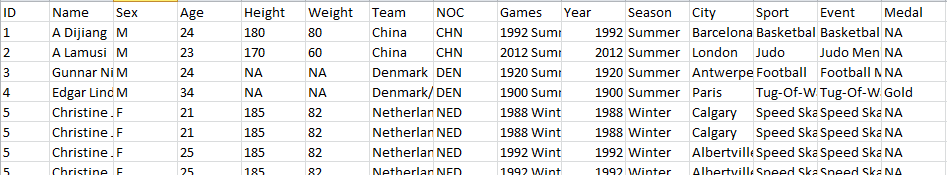
\includegraphics[width=0.95\textwidth, frame]
                        {./images/data/athlete_events.png} 
                    \caption{athlete\_events.csv}                  
                \end{figure}            
            \item NOC regions - A list of the countries and their NOC code. It is important to note some countries changed their code in the data. This is noted in Appendix A. 
                \begin{figure}[H]
                    \centering
                    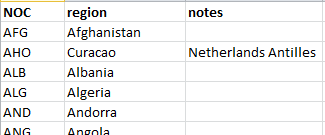
\includegraphics[width=0.6\textwidth, frame]
                    {./images/data/noc_regions.png}   
                    \caption{noc\_regions.csv}                 
            \end{figure}
        \end{enumerate}

    \subsubsection{Country Information}
    The second set of data relates to the information about each country, including their GDP and population. The most trustworthy source for this data publicly available from World Bank national accounts data, and OECD National Accounts data files. The data is available from 1960 to present, and is accessed as separate files. 
        \begin{enumerate}
            \item GDP - The GDP for all countries, represented in current US\$.
                \begin{figure} [H]
                    \centering
                    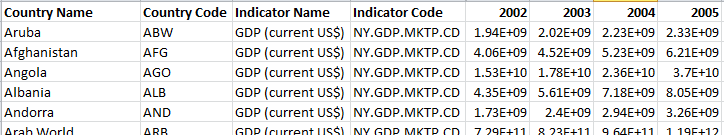
\includegraphics[width=0.95\textwidth, frame]
                        {./images/data/worldbank_gdp.png}
                        \caption{worldbank\_gdp.csv}                    
                \end{figure}
            \item Population - The total population of all countries.
                \begin{figure} [H]
                    \centering
                    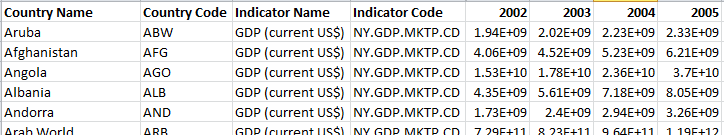
\includegraphics[width=0.95\textwidth, frame]
                        {./images/data/worldbank_gdp.png}      
                        \caption{worldbank\_gdp.csv} 
                \end{figure} 
        \end{enumerate}

    \subsubsection{Host Cities}
    The finally set of data is location of each of the games. The 'City' is included as a column in 'athlete\_events.csv', however it is not paired with a country which is needed to compare an athlete's country with where they are competing. This data was not readily available as a data file but the information was found on \url{https://architectureofthegames.net/olympic-host-cities/}. The data was copied into two separate text files as is; summer and winter. Using python the files were read, reformatted and combined to create a csv file. The NOC was also added as an additional column manually using noc\_regions.csv. The file contains the year, city, country, NOC and season of each Olympic games. The code is in Appendix A.1.
        \begin{figure} [H]
            \centering
            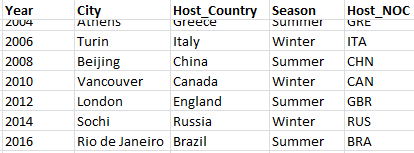
\includegraphics[width=0.6\textwidth, frame]
            {./images/data/host_countries.png}  
            \caption{host\_countries.csv}                  
        \end{figure}  

\subsection{Data Parsing}
    \subsubsection{Combined Dataset}
    From all of the above files, a new dataset was created using pandas (and article research) to refine the data selection, remove redundancies, combine related variables and update incorrect data to ensure a cleaner dataset for the visualisations. The code can be found in Appendix A.2. These steps were taken to combine the athlete\_events.csv, host\_countries.csv and noc\_regions.csv:
        \begin{enumerate}
            \item Remove 'Art Competitions' 
            \item Remove 'Name', 'Team' from athlete\_events.csv
                \begin{itemize}
                    \item 'Name' - the identification of the athletes is not important
                    \item 'Team' - sometimes contradicts NOC/Country
                \end{itemize}            
            \item Make NOC codes consistent for countries that have changed.            
            % EUA not in athlete_events
            % ROC already accounted for 
               \begin{itemize}
                    \item Singapore (SIN): Stored as SGP in athlete\_events
                    \item Russia (RUS): URS (1952-1988), EUN (1992), RUS (1994-2018)
                    \item Taiwan (TPE): ROC (1952-1976), TPE(1984-2018)
                    \item China (CHN): ROC (1924-1948), CHN (1980-2018)
                    \item Germany (GER): GER (1896-2018), EUA (1956-1964), FRG \& GDR (1968-1988)
                    \item Czech Republic (CZE): CZE (1994-2018), TCH (1920-1992), BOH (1900-1912)
                    \item Serbia (SRB): SCG (2004-2006), SRB (1912, 2008-2018), YUG (1920-2002)
                \end{itemize}            
            \item Add column COUNTRY by matching ‘NOC’ with the same from noc\_regions.csv
            \item Update host CITY in athlete\_events.csv to match more common names used in host\_cities.csv
                \begin{itemize}
                    \item Athina to Athens
                    \item Roma to Rome 
                    \item Antwerpen to Antwerp
                    \item Moskva to Moscow
                    \item Torino to Turin
                    \item Sankt Moritz to St Moritz
                \end{itemize}                 
            \item Add column HOST NOC by matching ‘NOC’ with same from host\_city.csv
            \item Add column for BMI using the formula Weight (kg) / Height\^2 (m) 
               \begin{itemize}
                    \item Height is in centimetres in the dataset so needs to be converted to metres (Height / 100)
                \end{itemize}
            \item Add column with Boolean value corresponding to whether an athlete is a medal winner     
            \item Add column GDP by matching ‘country’ in gdp.csv
                \begin{itemize}
                    \item File listed with years as columns
                    \item 'Melt' the table read in to create row entry for each NOC and year
                    \item Convert values to billions (divide by 1,000,000,000)
                \end{itemize}
            \item Add column POPULATION by matching ‘country’ in population.csv  
                \begin{itemize}
                    \item The same procedure as GDP
                    \item Convert the values to millions (divide by 1,000,000)
                \end{itemize}
        \end{enumerate}
    
        \begin{figure} [H]
            \centering
            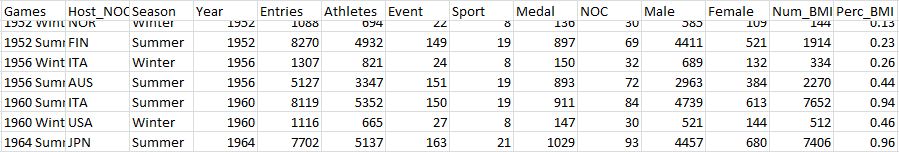
\includegraphics[width=0.95\textwidth, frame]
                {./images/data/games_draft.png}     
            \caption{games\_total\_draft.csv}               
        \end{figure} 

    At this point, the data was looking at more intensely and some preliminary graphs were tested. After reviewing this information, there were a few additional changes to be made. 
        \begin{enumerate}
            \item Remove Years 1896-1952 from athlete\_events.csv
                \begin{itemize}
                    \item Women didn't compete in 1896
                    \item Winter Games didn't commence until 1924
                    \item China and USSR joined in 1952
                    \item The recording of more than 40\% of weight and height started in 1956. Over 90\% since 1960.
                    \item The GDP and population is not available until 1960
                \end{itemize}
            \item Remove 'Winter' season, as not only will this overcomplicate the results and comparisons, but also Summer has a lot more data which will skew the outputs.
                \begin{itemize}
                    \item Summer has 2.3 times more countries each year
                    \item Summer has 2.3 times more sports each year
                    \item Summer has 4 times more athletes competing
                    \item summer has 3 times more events
                \end{itemize}
            \item Remove 'Season' and 'Games' columns   
                \begin{itemize}
                    \item Season is no longer relevant since only looking at Summer
                    \item Games was unique identifier between seasons, without season comparison it is just a duplicate of Year and Season
                \end{itemize}             
        \end{enumerate}

    With these changes, a new table was created with just Summer Olympics from 1956 with the above data. The code for this process is in Appendix A.2.      
        \begin{figure} [H]
            \centering
            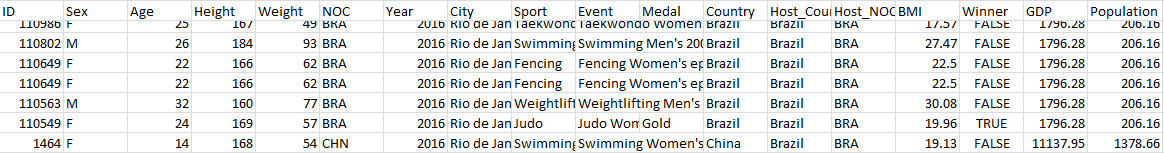
\includegraphics[width=0.95\textwidth, frame]
                {./images/data/all_data.png}      
                \caption{all\_data.csv} 
        \end{figure}

    \subsubsection{Totals}
    To adequately explore the summer dataset there were a number of aggregations that needed to be performed to calculate the total values of certain variables. Using panda data frames new subsets of the data were created to allow repeated access to these aggregations. The code is in Appendix A.3.
        \begin{enumerate} 
            \item \textbf{The Athletes} - This subset was created to refine the information relating to the individual athletes. This dataset is not considered with the type of sports or events the athlete participates in nor the year. 
                \begin{itemize}
                    \item Group the athletes by their ID so there is only one row per athlete, rather than a row for each entry by that athlete
                    \item Count the number of different sports the athlete competes in
                    \item Count the number of entries the athlete has in the summer dataset
                \end{itemize}
                \begin{figure} [H]
                    \centering
                    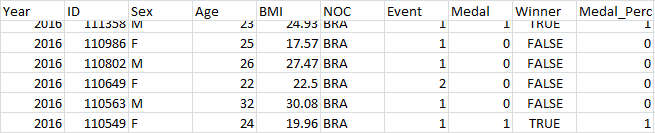
\includegraphics[width=0.95\textwidth, frame]
                        {./images/data/athlete_total.png}      
                        \caption{athlete\_total.csv} 
                \end{figure}

            \item \textbf{The Games} - This table breaks down the data into one entry per Games. It records the year and host country as well as the number of entries, events, sports, athletes (also broken down into Male and Female) and medals (also split into host and visitor amounts and percentages.)
                \begin{itemize}
                    \item Group the entries by the year, so there is only one entry per games
                    \item Keep column with Host Country Code
                    \item Count the number of entries for that year, store as 'Entries'
                    \item Count the number of athletes for that year (only one entry per athlete ID) as 'Athletes'
                    \item Count the number of unique events held that year as 'Event'
                    \item Count the number of unique sports hosted that year as 'Sport'
                    \item Count the number of medals awarded that year as 'Medal'
                    \item Add column 'Host\_Medal' to record the number of medals awarded to the host country
                    \item Add column 'Visitor\_Medal' to records all medals not awarded to host (total - host)
                    \item Count how many male athletes entered as 'Male'
                    \item Count how many female athletes entered as 'Female'
                    \item Calculate the percentage of medals awarded to the host
                    \item Calculate the percentage of medals awarded to all others
                \end{itemize}
                \begin{figure} [H]
                    \centering
                    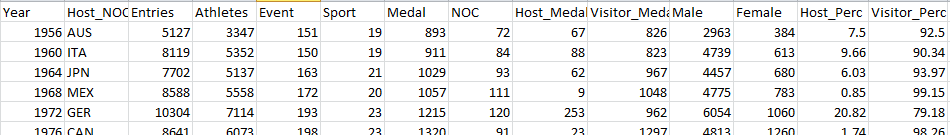
\includegraphics[width=0.95\textwidth, frame]
                        {./images/data/games_total.png}      
                        \caption{games\_total.csv} 
                \end{figure}

            \item \textbf{The Countries} - Finally, this dataset looks at the data from the perspective of the countries participating. There is an entry for each country and each games they compete it. As well as their code and name, this table also includes the GDP and population for the year, whether they were the host that year, as well as the same information as the games, except country specific.
                \begin{itemize}
                    \item Group the entries by the year and country code
                    \item Keep column with country code, name, GDP, population and whether they were the host 
                    \item Count the number of entries for that year, store as 'Entries'
                    \item Count the number of athletes for that year (only one entry per athlete ID) as 'Athletes'
                    \item Count the number of unique events held that year as 'Event'
                    \item Count the number of unique sports hosted that year as 'Sport'
                    \item Count the number of medals awarded that year as 'Medal'
                    \item Count how many male athletes entered as 'Male'
                    \item Count how many female athletes entered as 'Female'
                    \item Include number of medals and entries for each games
                    \item Calculate the percentage of medals awarded to the country from the total
                    \item Calculate the percentage of entries from the country compared to the total
                    \item Calculate the average number of events per athlete to determine uniqueness
                    \item Add column of Boolean whether country is in top 20 of total medals since 1956
                    \item Add column of Boolean whether country is in top 10 of total medals since 1956
                \end{itemize}
                \begin{figure} [H]
                    \centering
                    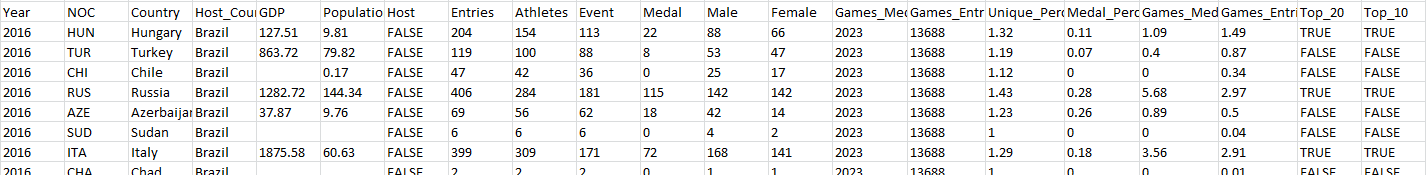
\includegraphics[width=0.95\textwidth, frame]
                        {./images/data/noc_total.png}      
                        \caption{noc\_total.csv} 
                \end{figure}

            \end{enumerate}



\section{Discussion}
The prediction of medal winners will be explored through a number of topics. Due to the difference n data size and added complexity, as explained in the data section, only data from the Summer Olympics since 1956 will be considered. The following questions will be explored and discussed.
            \begin{itemize}
                \item How have the games changed?
                \item What are the characteristics of an Olympic Athlete?
                \item Is there a difference in physicality between athletes and winners?
                \item Which countries are the best at the Olympics and how do they differ?
                \item Is the competition fair?
            \end{itemize}


    \subsection{The Games}
    There are many factors associated with the Olympic games including the number of entries, athletes (male and female), countries, events, sports and medals. The below histogram provides a sense of the distribution of these factors for all Modern Summer Olympics. A histogram is used to show how many occurrences there are of a single variable and grouping the data into bins (i.e. sets) to give a preliminary idea of the data. Additionally, the data was separated into two subgroups; games before and after 1955
        \begin{figure} [H]
            \centering
            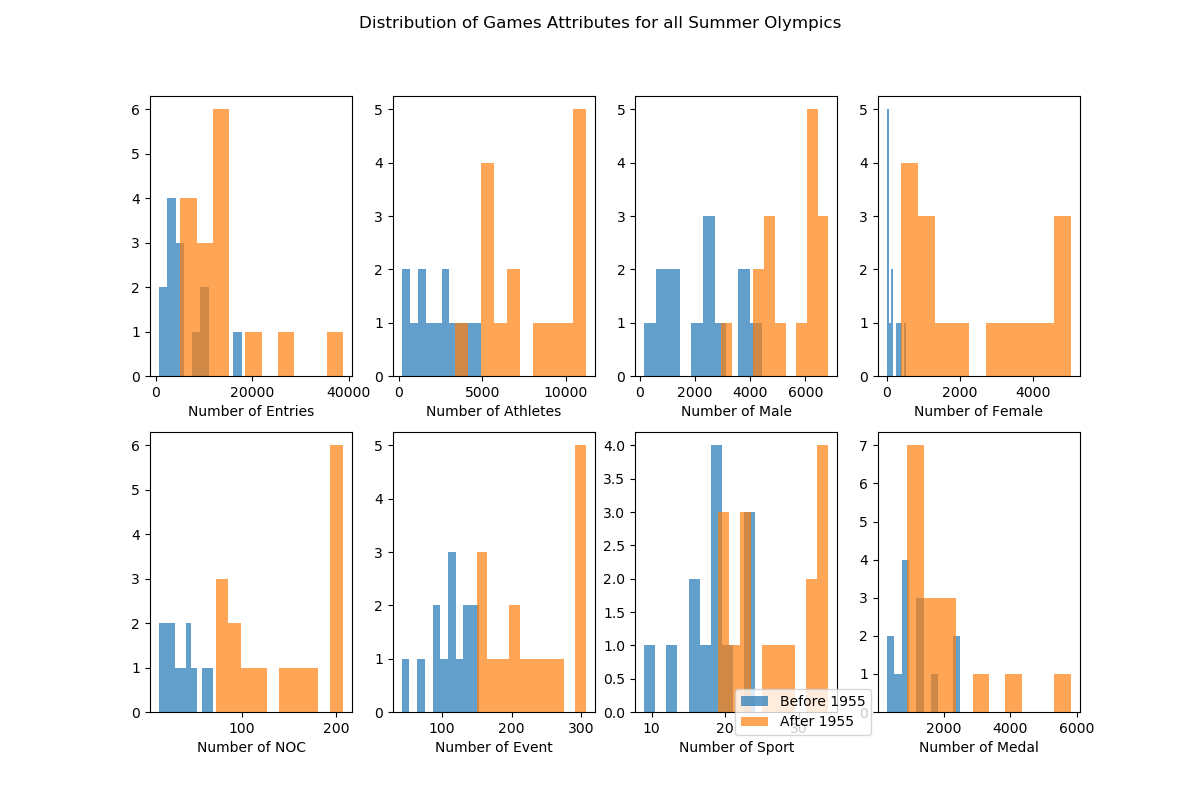
\includegraphics[width=\textwidth, frame]
                {./images/graph/games_histogram.png}      
                \caption{Distribution of variables in Games} 
        \end{figure}
    By doing so it is evident that the games have changed since the first 60 years of competition. All of the factors are considerably higher after 1955. Notably the number of women prior to 1955 was never higher than 500 competitors, but after this time, at least half of the games has seen more than 3,000 female competitors. Also, the number of countries competing has more than doubled with 6 of the games in the last 60 years seeing approximately 200 countries competing. From this graph it is evident that the Summer Olympic games have significantly diversified and become more accessible to more athletes around the world.

    \subsection{The Athletes}
    Without the athletes there would be no Olympic Games, so naturally the next topic to explore is the characteristics of the Olympiads themselves. Besides their country and their sport of choice, the defining characteristics of an athlete are their Age and BMI. Other interesting factors include how many events they compete in and how many medals on average an athlete wins.
    
    Firstly, the below boxplot shows the central tendency of athlete's age over the last 60 years of games. Additionally, the data are split by an athlete's sex to show the difference between male and female over time. A boxplot shows the spread of data as a compact alternative to a histogram, that highlights the general nature of the data. It identifies the median, 25th percentile and 75th percentile as the box, as well as low and high adjusters with outliers consistently. 
        \begin{figure} [H]
            \centering
            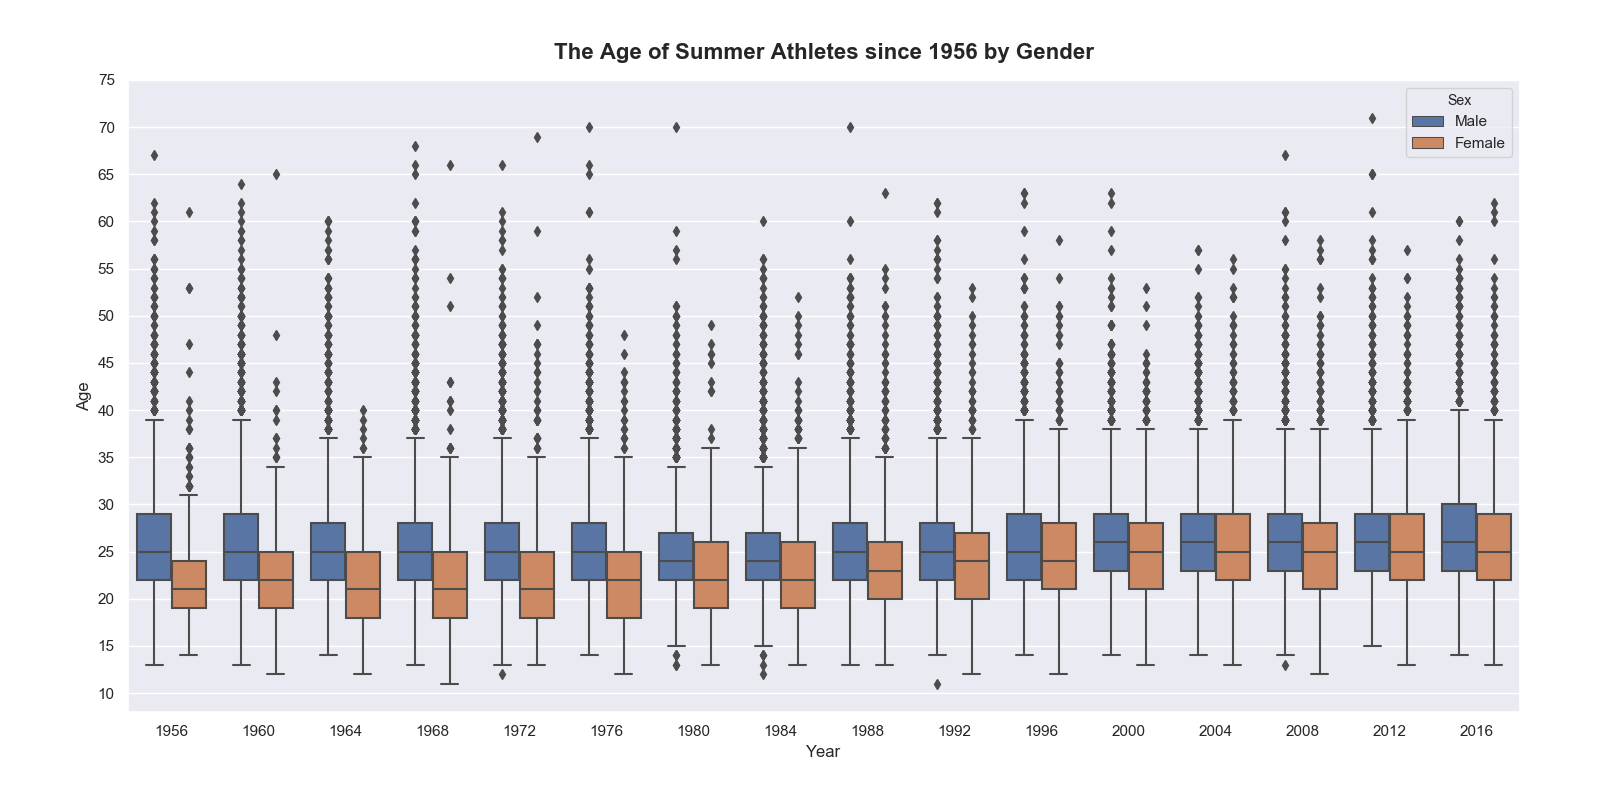
\includegraphics[width=\textwidth, frame]
                {./images/graph/athlete_age_boxplot.png}      
                \caption{Distribution of Age of Athletes by Year} 
        \end{figure}
    From this boxplot it is evident that the age and BMI of athletes has remaining fairly consistent through ....

    



    \subsection{The Athletes}

    \subsection{The Countries}





    \begin{itemize}
        \item The distribution of the number of events and medals [Histogram (\#events, \#medal)]
        


        
        \item The change in age for medal and non-medal winners [Turkey box (year v. age)]
        \item The BMI of medal and non-medal winners [q-q plot (medal v. non-medal BMI)]
        \item The proportion of medal winners to number athletes [scatter (\#athletes v. \#medals)]
        \item The proportion of men and women competing [scatter (\#females v. \#males)]
        \item The difference in \% of medals when competing at host [scatter (\% hosting v. visiting)]
        \item The effect of population and GDP on number of medals [multi \- pop, GDP, \#medals]
    \end{itemize}




% Appendix
\pagebreak
\appendix
\addappheadtotoc
\appendixpage
\section{Important notes about the data}
    \begin{enumerate}
        \item athlete\_events.csv - Possible factors that may affect results of each Olympics
            \begin{itemize}
                \item 1924: Winter games commence
                \item 1928: Women now compete in more than 2 sports
                \item 1932: Low attendance due to Great Depression
                \item 1940 \& 1944: Cancelled due to WW2
                \item 1948: Art sports (architecture, literature, music, painting, sculpture) removed
                \item 1952: USSR/Russia starts competing, Republic of China (ROC) discontinued
                \item 1956: Boycotts by 8 nations, including China
                \item 1960: Height and Weight measured consistently from now
                \item 1976: Boycotts by 25 nations (mostly from Africa)
                \item 1980: Boycotts by 66 nations, including US
                \item 2000: Summer Olympics capped at 28 sports, 300 events, 10,000 athletes                
            \end{itemize}

        \item noc\_regions.csv - The following countries are recorded under multiple codes:
            
        \begin{itemize}
                \item Australia: AUS, ANZ (New Zealand, 1908\-1912)
                \item Russia: URS (1952\-1988), EUN (1992), RUS (1994\-2018)
                \item China: ROC (1924\-1948), CHN (1952\-2018), HKG (Hong Kong, 1952\-2018)
                \item Germany: GER (1896\-2018), EUA (1956\-1964), FRG \& GDR (1968\-1988)
                \item Czech Republic: CZE (1994\-2018), TCH (1920\-1992), BOH (1900\-1912)
                \item Serbia: SCG (2004\-2006), SRB (1912, 2008\-2018), YUG (1920\-2002)                    
            \end{itemize}  

    \end{enumerate}





\pagebreak
\appendix
\appendixpage
\addappheadtotoc
\section{About the data}

\subsection{Host Cities}
\lstinputlisting[language=python]{code/host_countries.py}

\pagebreak
\subsection{Combined Data}
\lstinputlisting[language=python]{code/all_data.py}

\pagebreak
\subsection{Combined Data}
\lstinputlisting[language=python]{code/totals.py}









\end{document}